% Copyright 2018 Sebastian B. Galkin

% This file is part of paraseba/scaladores-may-2018-talk.

% paraseba/scaladores-may-2018-talk is free software: you can redistribute it and/or modify
% it under the terms of the GNU General Public License as published by
% the Free Software Foundation, either version 3 of the License, or
% (at your option) any later version.

% paraseba/scaladores-may-2018-talk is distributed in the hope that it will be useful,
% but WITHOUT ANY WARRANTY; without even the implied warranty of
% MERCHANTABILITY or FITNESS FOR A PARTICULAR PURPOSE.  See the
% GNU General Public License for more details.

% You should have received a copy of the GNU General Public License
% along with Foobar.  If not, see <http://www.gnu.org/licenses/>.

\begin{center}
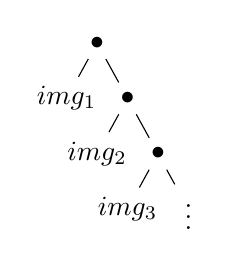
\begin{tikzpicture}[sibling distance=2.2em, level distance=2em]
  \node {\(\bullet\)}
    child { node {\(img_1\)} }
    child { node {\(\bullet\)}
      child { node {\(img_2\)}}
      child { node {\(\bullet\)}
        child { node {\(img_3\)}}
        child { node {\(\vdots\)}
    }}};
\end{tikzpicture}
\qquad
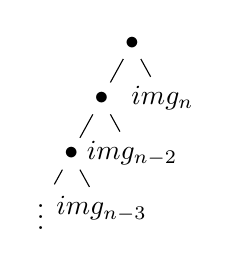
\begin{tikzpicture}[sibling distance=2.2em, level distance=2em]
  \node {\(\bullet\)}
    child { node {\(\bullet\)}
      child { node {\(\bullet\)}
        child {node {\(\vdots\)}}
        child {node {\(img_{n-3}\)}}}
      child { node {\(img_{n-2}\)}}
        }
    child { node {\(img_n\)} };
\end{tikzpicture}
\qquad
\begin{tikzpicture}[level distance=2em, level 3/.style={sibling distance=3em}, level 2/.style={sibling distance=2.5em}, level 1/.style={sibling distance=6em}]
  \usebeamercolor{example text}
  \node {\(\bullet\)}
  child { node[color=fg] {\(\bullet\)}
    child { node[color=fg] {\(\bullet\)}
      child {node[color=fg] {\texttt{zero}}}
      child {node[color=fg] {\(img_1\)}}}
    child { node[color=fg] {\(img_2\)}}
  }
  child { node[color=red] {\(\bullet\)}
    child { node[color=red] {\(img_3\)} }
    child { node[color=red] {\(\bullet\)}
      child { node[color=red] {\(img_4\)}}
      child { node[color=red] {\(\vdots\)}
      }}};
\end{tikzpicture}
\end{center}